\section{Proposed Research Activity}
\label{sec:research_activity}
After the presentation of the context of interest and the aspects to be treated in the current research proposal, this section will formalize the hypotheses reported in Section \ref{sec:research_topic}, identifying the methods of interest and the procedures that will be used to validate and compare the proposed approach against the state-of-the-art methods.
Building upon the discussion presented in Section \ref{sec:research_topic}, a pertinent question emerges. In scenarios where a robot is required to perform a task based on a provided command, \textit{``How can we enhance the robot's cognitive capabilities to accurately interpret the given command?"} This question becomes particularly relevant in light of our observation that a significant challenge lies in the system's proficiency to precisely identify the target object as specified in the command. As a result, our research centers on the task of accurately identifying the target object within the agent's surroundings when provided with a desired command.
\newline In literature, there are recent \textit{Imitation Learning methods}, that follow an object-oriented paradigm \cite{park2021object, belkhale2023plato, zhu2023viola, jiang2023vima}. However, methods like \cite{belkhale2023plato} primarily focus on learning the affordance of individual objects, taking in input the current observation and the desired state of a specific object. On the other hand, techniques in the field of vision-based manipulation, such as \cite{zhu2023viola, jiang2023vima}, leverage pre-trained object detectors like Mask-RCNN \cite{he2017mask}. These detectors identify the top-k predicted bounding-boxes that \textbf{potentially contain objects} in the scene and use this information to infer the appropriate actions. In contrast to these methods, our approach draws inspiration from Computer Vision tasks like ``Vision Question and Answering" also known as ``Visual-Scene Reasoning" \cite{perez2018film}. In this task, the system is responsible for generating an answer to a given query (e.g., a textual representation of a question) based on an input image. What distinguishes this approach is its capability to \textbf{selectively focus on specific segments of the image}, guided by the content of the question, as illustrated in Figure \ref{fig:film_attention}
\begin{figure}[htb]
    \centering
    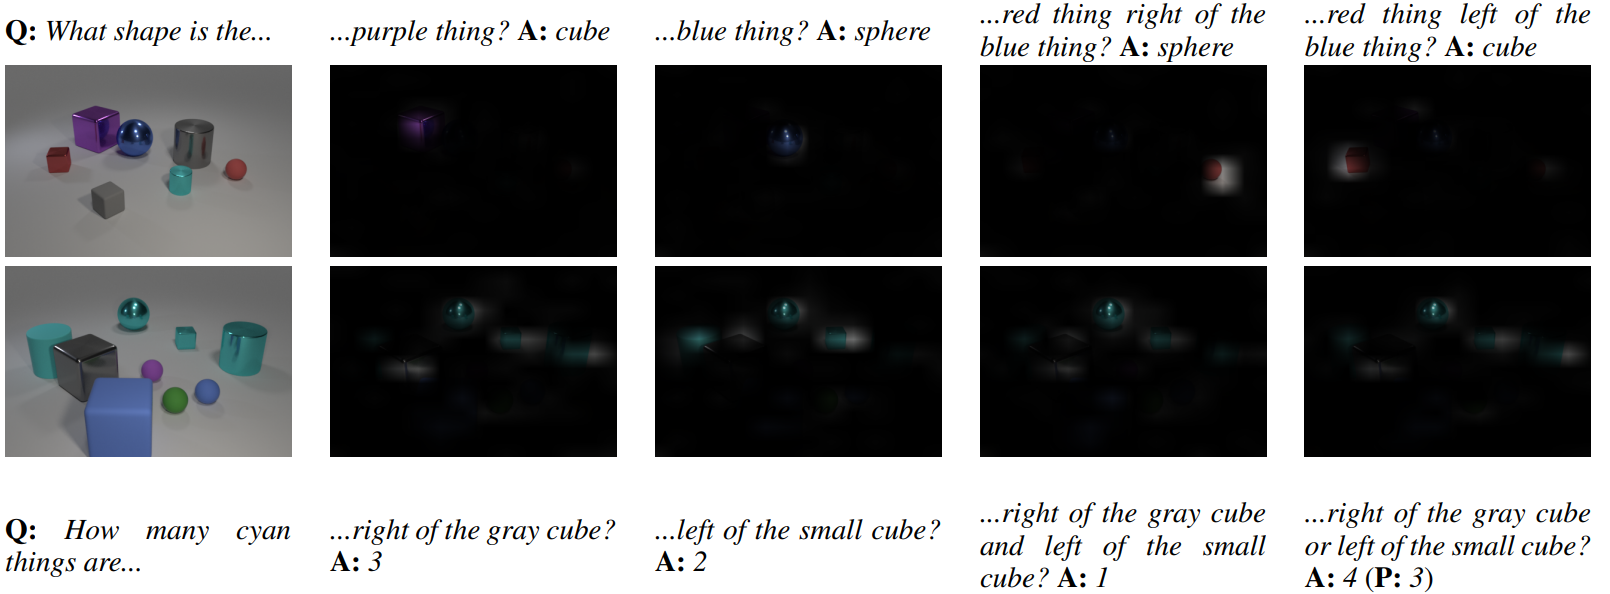
\includegraphics[width=0.9\textwidth]{Figures/images/film/film_attention.png}
    \caption{\textit{Vision Question and Answering task}, starting from a an image and a text, the method is able to generate an answer by focusing on specific part of the image based on the question.}
    \label{fig:film_attention}
\end{figure}


In conclusion, our proposal aims to explicitly address the \textbf{cognitive aspect} of task understanding by introducing a dual-stage system. The first stage focuses on command analysis and understanding, while the second stage tackles action generation based on information from the first module. Given the challenge of accurately identifying the target object, we introduce a \hl{\textit{Conditioned-Target \ Object \ Detection \ task}},\change{\small Definizione di tutti gli elementi } where the system identifies the target object location by predicting its bounding-box, $bb_{t}^{target} \in \mathbb{N}^{4}$, defined as vector of 4 integer elements $[x^{upper-left},y^{upper-left}, x^{bottom-right}, y^{bottom-right}]$ representing the coordinates in pixel of the upper-left and bottom-right corners. \hl{The inputs are the current image observation $s_{t} \in \mathbb{R}^{H \times W \times 3}$ and the command $c_{m_{i}} \in \mathbb{R}^{T \times H \times W \times 3}$ expressed as demonstration video, i.e., $bb_{t}^{target} = \mathcal{F}_{\psi}(s_{t}, c_{m_{i}})$}, where $\mathcal{F}_{\psi}$ is a parametrized function approximator such as Deep Neural Network. \hl{This approach should \textbf{simplify} the action-inference process, as the system benefits from \textbf{explicit \ low-level  \ information} about the objects to be manipulated}. \hl{The overall goal is to enhance the system's performance by breaking down the task into distinct stages, improving cognitive task understanding, and streamlining subsequent action generation}.\change{\small Pros della proposta}

In order to validate the hypothesis that following a modular approach can affect positively the system performance, we will follow an incremental approach, divided into 4 main steps:
\begin{enumerate*}[label=(\arabic*)]
    \item \textbf{Baseline definition}, this initial step is crucial to establish a baseline and point out critical aspects of the current state-of-the-art methods;
    \item \textbf{Incorporate ground-truth information into the baseline's control module}, after assessing the baseline, the second phase focuses on empirically assessing whether adding target-object information to the control modules can enhance system performance. During this phase, to prevent \textit{error propagation}, the control module will receive input based on ground-truth information;
    \item \textbf{Development of a Conditioned-Target Object Detector System}, once the second step is completed, we can formulate the Conditioned-Target Object Detector problem and evaluate its efficacy in addressing the tasks at hand;
    \item \textbf{Integration of the developed system with the baseline}: After achieving a stable system in the previous step, we will integrate the developed system with the baseline architecture to assess overall system performance
\end{enumerate*}

In the initial iteration, the methods will undergo training in a Single-Task Multi-Variation scenario, i.e., we consider single-task such as pick-place and nut-assembly, each task composed of different variations (Figure \ref{fig:mosaic_tasks}). Subsequently, leveraging the class-agnostic property, the system will be extended to a Multi-Task scenario.
Preliminary experiment will be performed in simulation, then a real-world dataset will be collected and used to train models to be validated on a real-robot setup.
Results and additional details concerning these problems will be presented in Chapter \ref{chapter:preliminary_results}."
% \newline As discussed in Section \ref{sec:research_topic}, it was seen that current methods start from a representation of the environment that lacks geometric information and that is obtained from the point of view different from that of the robot, and in particular from that of the end-effector. 
% Concerning this point, starting from the state-of-the-art architecture \cite{mandi2022towards_more_generalizable_one_shot} based on Transformer, the goal will be to extend it in such a way that it will be able to handle time sequences characterized by RGB-D observations, and taken from a camera mounted on the end-effector. Several approaches can be used to achieve this. In fact, in the Computer Vision community, RGB-D images can be handled in different ways. For example, one can apply convolutional layers separately on the RGB and depth images, as in \cite{zhang2018deep_vr_teleoperation}, and subsequently perform a fusion between the extracted features based, for example, on their concatenation. Another approach may be using a 3D Point-Cloud Neural Network, such as \cite{qi2017pointnet++} used in \cite{fang2020graspnet}. To answer the question which of the two approaches to prefer, given that the reference method \cite{mandi2022towards_more_generalizable_one_shot} has a transformer-based architecture, a first step may be to apply convolutional filters separately on the RGB and D images and then combine them appropriately, going on to evaluate different fusion techniques, starting from simple concatenation to the use of a weighted sum, with the ultimate goal of generating the embedding as input to the transformer.
% \newline This setting will allow evaluating the hypothesis that adding geometric information can reduce failures caused by collisions with objects of interest or by the inability to determine when to close or open the gripper.  
% The resulting method will then be tested and compared first in simulation, taking advantage of the open-source simulation environments \cite{brockman2016openai,zhu2020robosuite}. Then, based on the obtained results, the proposed architecture will be tested and evaluated on a real robot platform, adding an additional experimental contribution that current methods such as \cite{dasari2021transformers_one_shot,mandi2022towards_more_generalizable_one_shot} lack.
% \newline As for the tasks of interest, the main focus will be devoted to industrial tasks (e.g., pick-and-place, push, peg-insertion), introducing an additional constraint with respect to \cite{mandi2022towards_more_generalizable_one_shot}, since the system will have to be able to perform real-time inference on low-cost embedded platforms, in order to control a real-world robot platform.
% \newline An incremental approach will be used for the design and development of the proposed system. Thus, a single-task setting will first be evaluated, but, with respect to \cite{mandi2022towards_more_generalizable_one_shot}, it will be characterized by a high degree of variability based on different initial conditions and different objects to be manipulated so as to evaluate the ability to generalize across a single task, a setting in which meta-learning-based procedures have proven successful \cite{finn2017one_shot_visual_il,yu2018daml}. Next, the system will be extended into a multi-task context, where the hypotheses made earlier about using Variational-Autoencoder for learning a representation related to the demonstrated sub-tasks can be evaluated and validated in combinations with the use of Contrastive Loss, which have been shown to be valid in methods such as \cite{sermanet2018time_contrastive,zakka2022xirl} where the goal has been to learn a task representation from different embodiments \cite{zakka2022xirl} and different viewpoints \cite{sermanet2018time_contrastive}. Here, with respect to \cite{Mandlekar2020GTI}, the Variational Autoencoder will be combined with Contrastive Loss, to learn a sub-task related representation starting from demonstrations composed of different visual appearance. While, with respect to \cite{mandi2022towards_more_generalizable_one_shot}, the proposed combination aims to model explicitly the concept of sub-tasks, which may help the generalization in a multi-task settings by leveraging the task hierarchical structure.
